\section{Methods}
\label{sec:methods}

\subsection{Datasets}
\label{sec:methods:data}

Our primary analysis uses two publicly available kinase inhibitor profiling
datasets, described first. Two further datasets are added below to confirm the
findings across additional assay technologies.
The Davis dataset\cite{Davis2011} is comprised of binding affinities ($K_d$) for 68
small-molecule kinase inhibitors measured against 433 human kinase domains.
Affinity values are reported as dissociation constants and were converted to
$\mathrm{p}K_d = -\log_{10}(K_d / 10^9)$ prior to analysis, following the
convention of the DeepDTA benchmark.\cite{DeepDTA}
% Pairs for which no binding was detected at the screening concentration of
% 10~$\mu$M were assigned $\mathrm{p}K_d = 5.0$, corresponding to a $K_d$ of
% 10~$\mu$M, which represents the detection floor of the assay.
The resulting affinity matrix is complete ($68 \times 433$, 29{,}444 entries),
with all non-binding pairs assigned the detection-floor value
$\mathrm{p}K_d = 5.0$ (corresponding to a $K_d$ of 10~$\mu$M).
This is the standard convention for the dataset\cite{DeepDTA,Bosc2017} and
slightly underestimates true non-binding affinity.

Active entries (pKd $> 6$, i.e.\ $K_d < 1~\mu$M) make up 17.9\% of the Davis
matrix. This cutoff answers ``was binding detected above assay noise/floor,''
the conventional boundary used in kinase profiling, rather than ``is this
target plausibly occupied at physiological drug concentrations,'' a question
affinity values alone cannot answer without exposure data (e.g.\ free-drug
concentration) that neither dataset provides. A stricter cutoff
($\mathrm{p}K_d \geq 7$, $K_d < 100$~nM) leaves the agreement between
selectivity definitions unchanged but shrinks per-compound active sets,
pushing more compounds toward the zero/near-zero-active regime that
Section \ref{sec:results:instability} identifies as least rank-stable. 

The Klaeger dataset\cite{Klaeger2017} is comprised of binding affinities for 243
clinical kinase inhibitors profiled against the human kinome using
Kinobeads chemical proteomics.
Apparent dissociation constants ($K_d^\mathrm{app}$) were derived from
dose--response curves across eight inhibitor concentrations in cancer cell
lysates.
Only high-confidence measurements (as annotated by the original authors) were
retained, yielding 5{,}123 drug--target pairs for 222 drugs and 343 kinase
targets.
Affinity values were converted to $\mathrm{p}K_d$ using the same formula as
above.
Missing entries, representing kinase--inhibitor combinations not detected in
the assay, were assigned the background value $\mathrm{p}K_d = 5.0$.
The resulting Klaeger matrix is $222 \times 343$.
Active entries (pKd $> 6$) make up 3.6\% of the Klaeger matrix, versus 17.9\%
for Davis above.
The lower active fraction for Klaeger reflects the more stringent detection
threshold of the chemoproteomic assay.

To test whether our findings depend on the assay technology, we added two
further datasets that measure kinase inhibition by different means.
The Anastassiadis dataset\cite{Anastassiadis2011} profiles 178 inhibitors
against 300 kinases in a single-concentration ($0.5~\mu$M) radiometric activity
assay, reported as percent residual kinase activity relative to a solvent
control.
We converted these to percent inhibition ($100$ minus residual activity,
clipped to $[0,100]$, where higher values denote stronger inhibition), with the
$1.1\%$ missing entries set to zero inhibition.
The Metz dataset\cite{Metz2011} reports $\mathrm{p}K_i$ affinities for a large
medicinal-chemistry
campaign using the same negative-log scale as $\mathrm{p}K_d$. The value
$\mathrm{p}K_i = 4.0$ is the lowest value reported anywhere in the released
data (only $0.17\%$ of measurements), so we assign it to unmeasured
combinations as the assay's own detection floor (the same convention used for
the Davis $\mathrm{p}K_d = 5.0$ floor above). Coverage per compound is highly
skewed (a median compound is measured against only 21 of the 172 kinases), so
we restricted the dataset to the 704 compounds profiled against at least 50 of
the 172 kinases, keeping profiles in which most entries reflect a real
measurement rather than floor imputation while retaining a large enough
compound set for the panel-size and instability analyses.

The four datasets span three assay technologies (competition binding,
chemoproteomics, and functional activity) and two readout types (affinity and
single-concentration inhibition).
Each selectivity definition is computed on the native readout of its
dataset, and our analyses concern rank correlations between definitions and rank
instability. Figure~\ref{fig:fidelity} shows the definitions are not 
invariant to the choice of readout. In fact, two defensible
operationalizations of the entropy rank compounds differently, and on Klaeger in
reverse. Cross-dataset comparison here rests on rank correlations computed within
each dataset, never on absolute scores compared across them.
For the percent-inhibition and $\mathrm{p}K_i$ datasets, the S-score threshold, and
entropy/Gini baseline grids were shifted to span each dataset's active range,
while the ratio off-target index $k \in \{1,\ldots,5\}$ was left unchanged
(it is an index of off-targets and so needs no rescaling).

We excluded two additional candidate datasets.
The Gao screen\cite{Gao2013} is a single-concentration functional inhibition
assay of the same readout type as the Anastassiadis dataset already included,
and its raw data are not openly redistributable. Including it would add a
second instance of an assay type rather than a new assay technology.
The Patricelli study\cite{Patricelli2011} profiles only a small number of
inhibitors against native kinases as a proof of concept for the KiNativ
platform. A ranking-stability analysis requires many compounds to produce a
meaningful ranking, so this dataset is not suited to the present comparison.

\subsection{Selectivity Definitions and Parameterization}
\label{sec:methods:defs}

We implemented four selectivity definitions, each including
parameters whose values are not standardized in the literature.
We discuss each definition below.
Throughout, a compound's binding profile is the vector of its affinities
$\mathrm{p}K_{d,i}$ across the $N$ panel kinases, with higher
$\mathrm{p}K_{d}$ denoting tighter binding.

\paragraph{S-score.}
Karaman et al.\cite{Karaman2008} defined the selectivity score as the fraction
of the panel that a compound inhibits: the number of kinases ``bound'' divided
by the number tested, where a kinase counts as bound when the compound reduces
its activity below a fixed cutoff at a single screening concentration (the
original work reports $S(35)$, $S(10)$ and $S(1)$ for cutoffs of $35\%$, $10\%$
and $1\%$ of control activity).
We implemented the same fraction, expressing the bound criterion as an affinity
threshold $\tau$ on $\mathrm{p}K_d$:
\begin{equation}
  S(\tau) = \frac{1}{N} \sum_{i=1}^{N} \mathbf{1}[\mathrm{p}K_{d,i} > \tau].
\end{equation}
Sweeping $\tau$ reproduces their family of cutoffs. We used
$\tau \in \{5.5, 5.75, \ldots, 8.0\}$ (11 values), spanning $K_d$ cutoffs from
approximately 3~$\mu$M to 10~nM.

\paragraph{Selectivity entropy.}
Uitdehaag and Zaman\cite{Uitdehaag2011} treat the compound's binding across the
panel as a probability distribution and report its Shannon entropy. A profile
concentrated on few kinases has low entropy and is selective.
In the original definition, the weight on each kinase is its association constant
$K_{a,i} = 1/K_{d,i}$ (the share of compound that would be bound to kinase $i$
in an equimolar mixture), so $p_i = K_{a,i}/\sum_j K_{a,j}$.
We implemented the entropy on the same log-affinity scale used by the other
metrics, weighting each kinase by its affinity in excess of a baseline $\beta$:
\begin{equation}
  H(\beta) = -\sum_{i=1}^{N} p_i \log_2 p_i, \quad
  p_i = \frac{\max(\mathrm{p}K_{d,i} - \beta,\, 0)}
             {\sum_j \max(\mathrm{p}K_{d,j} - \beta,\, 0)},
\end{equation}
where $\beta$ is the affinity below which binding is treated as negligible.
This makes $\beta$ an explicit parameter (its under-specification motivates
property D3 below). We swept $\beta \in \{5.0, 5.25, \ldots, 6.5\}$ (7 values),
a narrower range than the S-score's $\tau$ sweep above. Both parameters key off
the same threshold-crossing event, so sweeping either one far enough leaves a
growing share of compounds with no kinase above the cutoff (on Klaeger, 7.2\%
of compounds at $\mathrm{p}K_d = 6.0$ versus 55\% at $\mathrm{p}K_d = 8.0$),
degenerating the S-score toward an uninformative 0 and the entropy and Gini
weights toward an undefined 0/0 alike. The $\tau$ range 
(whose S-score is not necessarily immune to this) is wider because it was 
chosen to reproduce Karaman
et al.'s published cutoffs (approximately 3~$\mu$M to 10~nM). $\beta$ has no
equivalent published reference points and was kept closer to the
$\mathrm{p}K_d = 6$ active threshold used elsewhere in this work.
The association-constant and log-affinity weightings are distinct reasonable
choices that can rank compounds differently, which is itself an instance of the
definitional instability this paper characterizes. We quantify the difference
below. % (``Faithfulness to the original definitions'').

\paragraph{Gini coefficient.}
Graczyk\cite{Graczyk2010} adapted the Gini coefficient from economics: kinases
are sorted by activity and the cumulative fraction of total binding is plotted
against the cumulative fraction of kinases (a Lorenz curve). The Gini
coefficient, which measures how unequally is binding distributed across the kinome,
is twice the area between this curve and the diagonal of equal
distribution.
The original work computes it from percent-inhibition values.
As with the entropy above, implemented the entropy on the same log-affinity scale
for the same reason.
We applied the standard discrete Gini formula to that baseline-subtracted
log-affinity profile:
\begin{equation}
  G(\beta) = \frac{2\sum_{i=1}^{N} i \cdot x_{(i)}}{N \sum_{i=1}^{N} x_{(i)}} - \frac{N+1}{N},
  \qquad x_{(i)} = \max(\mathrm{p}K_{d,i} - \beta,\, 0)\  \text{sorted ascending}.
\end{equation}
We swept $\beta$ over the same range as for the entropy.
A compound whose binding is concentrated on one kinase has a highly unequal
distribution ($G$ is near 1), while a compound that binds many kinases equally has
$G$ near 0. Higher values therefore indicate greater selectivity.

\paragraph{Ratio.}
Classical pharmacological selectivity is pairwise. It quantifies how much more tightly a
compound binds its primary target than an off-target.
We implemented this as the fold-selectivity, in log units, between the primary
target and the $k$-th ranked off-target:
\begin{equation}
  R(k) = \mathrm{p}K_{d,(1)} - \mathrm{p}K_{d,(k+1)}
       = \log_{10}\frac{K_{d,(k+1)}}{K_{d,(1)}},
\end{equation}
where $\mathrm{p}K_{d,(j)}$ is the $j$-th largest affinity in the profile and
$k \in \{1, 2, 3, 4, 5\}$ selects the reference off-target. We capped $k$ at 5
because, on the sparser Klaeger panel, a large share of compounds already have
fewer than five active kinases (median 5.5; $45\%$ have fewer than five). For
those compounds, a larger $k$ would compare the primary target against the
assay floor rather than a genuine off-target.
$R(k)$ takes
the affinity gap to a single chosen competitor, the $k$-th ranked off-target.
The field also assigns the concentration- and target-dependent selectivity
(CATDS) score of Klaeger et al.\cite{Klaeger2017} to this family, though we find
that it does not behave like a member of it. CATDS divides each
target's concentration-dependent binding reduction by the sum of binding
reductions over \emph{every} target in the panel, rather than comparing to a
single chosen competitor, which is a distributional construction. We therefore
represent the ratio family by $R(k)$ alone and treat CATDS separately in the
Discussion.
We use the simpler fold-selectivity because the reference off-target index $k$
is then an explicit parameter whose effect can be studied directly.
A larger affinity gap to the nearest competitor means greater selectivity, so
higher $R(k)$ indicates greater selectivity.
% \emph{In words:} how big is the affinity gap between the primary target and the
% next-best one? A larger gap means greater selectivity.

\paragraph{Faithfulness to the original definitions.}
The S-score and the ratio are computed in the form given by their original
sources (a panel-hit fraction and a primary-to-off-target affinity ratio,
respectively).
For the entropy and the Gini coefficient, we used the baseline-subtracted
log-affinity profile in place of the original association constants (entropy)
and percent-inhibition values (Gini), so that all four metrics operate on one
common scale, and making baseline $\beta$ an explicit calculation parameter.
To confirm that this choice does not implicitly determine our conclusions, we
recomputed the entropy and Gini in forms closer to the originals
(association-constant weighting) and compared the resulting rankings with the
log-affinity forms.
The two operationalizations differ substantially: for entropy, Spearman
$r = 0.42$ (Davis) and $-0.32$ (Klaeger), while for Gini, $r = 0.11$ and $-0.45$
(Figure~\ref{fig:fidelity}). This confirms that the operationalization
of a named metric is a source of the definitional instability.

\begin{figure}[htbp]
  \centering
  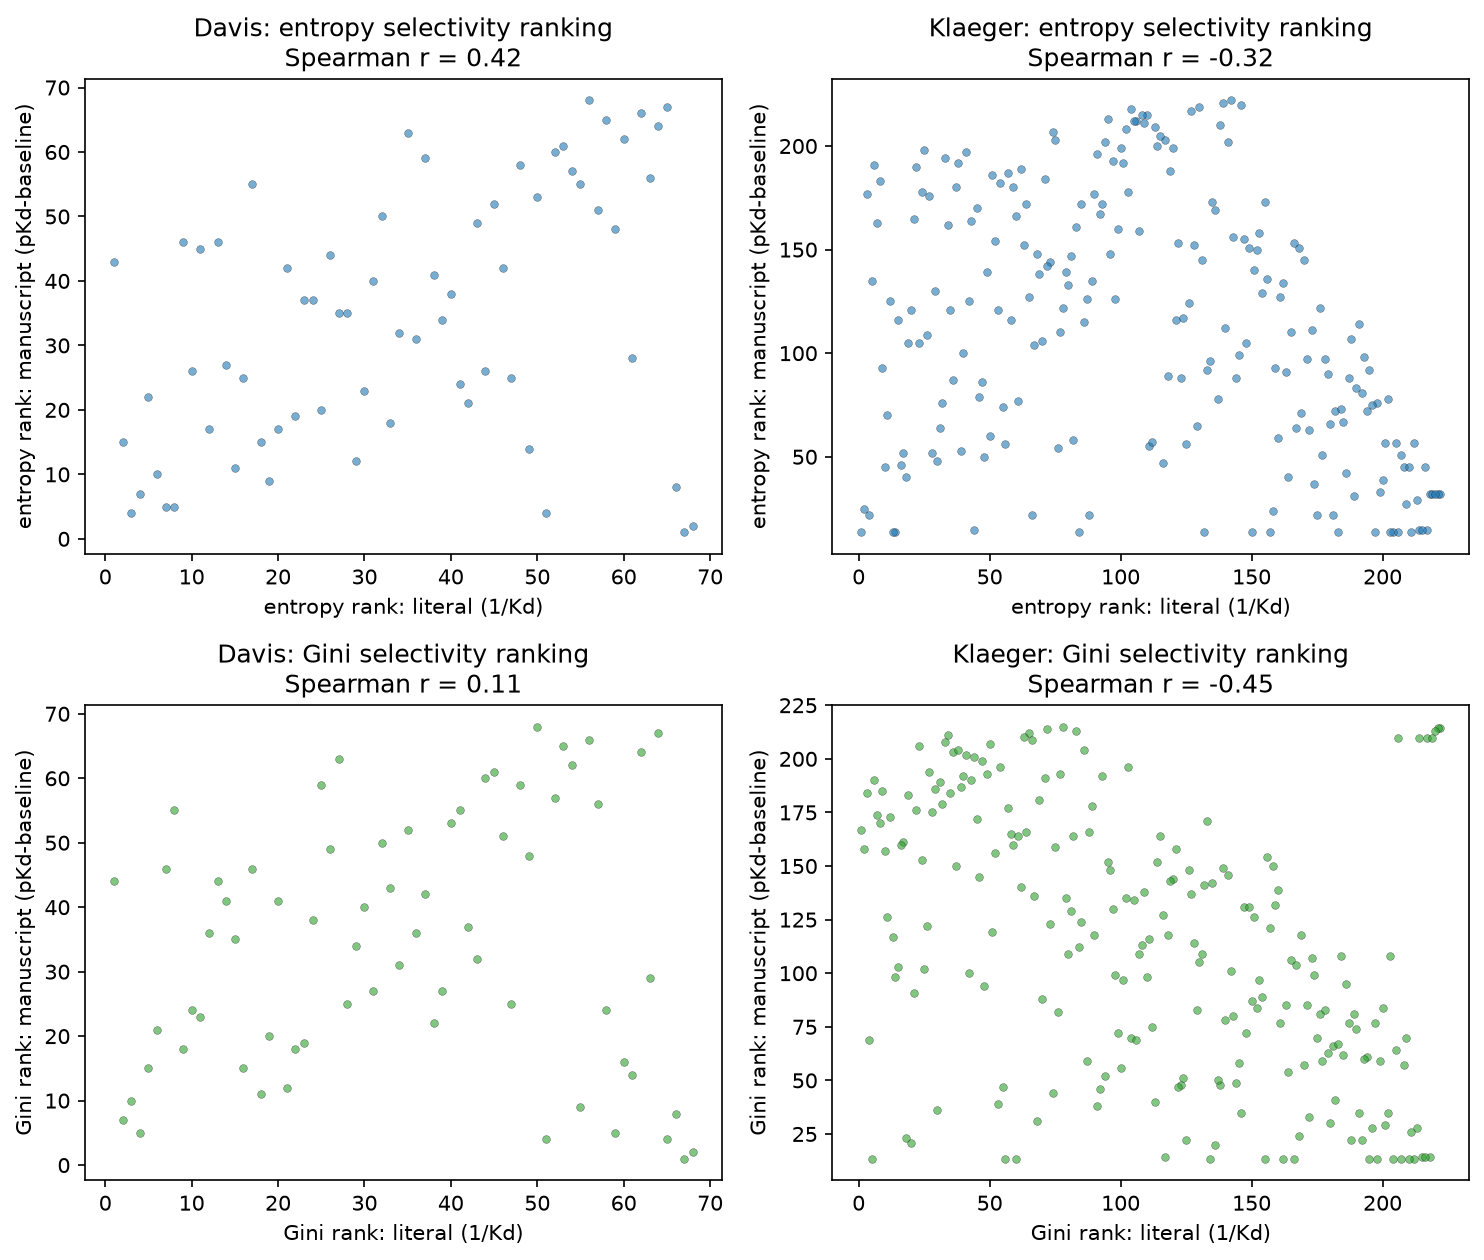
\includegraphics[width=\textwidth]{figures/metric_fidelity}
  \caption{Operationalization sensitivity of the entropy and Gini coefficient.
           For each dataset, the compound selectivity ranking computed in a form
           close to the original publication (association-constant weighting) is
           plotted against the baseline-subtracted log-affinity form used in the
           main text. Top row: selectivity entropy; bottom row: Gini coefficient.
           The two operationalizations of the same named metric differ
           substantially, and the entropy ranking even reverses on Klaeger,
           confirming that the operationalization of a named metric is a
           source of the definitional instability.}
  \label{fig:fidelity}
\end{figure}

\subsection{Rank Stability Analysis}
\label{sec:methods:stability}

For each definition and each parameter value, compounds were ranked from most
selective (rank 1) to least selective (rank $n$, where $n$ is the number of
compounds in the dataset).
Ties were broken by average rank.
This yielded 30 rank vectors per dataset for Davis, Klaeger, and Metz (11 for
the S-score, 7 for entropy, 7 for Gini, and 5 for ratio), and 28 for
Anastassiadis, whose coarser native percent-inhibition scale supports only 9
S-score threshold values rather than 11.

For each compound, rank instability was quantified as the standard deviation
of its rank across all configurations for that dataset (overall instability)
and separately
across parameter configurations within each definition family (within-family
instability).
Cross-definition-family agreement was assessed using Spearman rank correlation
between the median rank vectors of each definition family.
The median was taken across parameter values within each family, rather than
the mean, because the
median is less sensitive to the inclusion or exclusion of outliers than the mean.

Associations between rank instability and binding profile features were
assessed using Spearman correlation, restricted to the Klaeger and Davis
datasets. These are the two datasets on a $\mathrm{p}K_d$ scale, so the same
activity threshold and affinity-based features apply directly, allowing the
predictor structure to be checked for replication across a second dataset.
Profile features computed for each compound included: the number of active
kinases ($\mathrm{p}K_d > 6$), the gap between the top and second-ranked
affinities, the standard deviation and range of active affinities, and the
absolute affinity of the second-ranked target.
All correlations are reported with two-tailed $p$-values. Significance
thresholds of $p < 0.05$, $p < 0.01$, and $p < 0.001$ are denoted *, **, and
*** respectively.
Analyses were performed in Python 3.10 using NumPy, pandas, and
SciPy.\cite{NumPy,pandas,SciPy}
A secondary analysis relating selectivity rankings to clinical adverse-event
outcomes (FAERS report rates and FDA-label discontinuation rates for the
FDA-approved Klaeger compounds) is summarized in the Limitations section.
The analysis code and full per-definition results are available in the code
repository (see Data and Software Availability).
